\documentclass[spanish,9pt]{beamer}
\usetheme{tree}
%\usepackage{german}
\usepackage[latin1]{inputenc}
\usepackage[spanish]{babel}

% Images
\usepackage{graphicx}
\usepackage{multicol} 
\usepackage{subfigure} % subfiguras
\usepackage{caption}
\usepackage{float}
\captionsetup[table]{labelformat=empty}
\captionsetup[figure]{labelformat=empty}

\usepackage{amsmath}
\usepackage{amsfonts}
\usepackage{dsfont}
\usepackage{parskip}
\usepackage{hyperref}

\usepackage{listings}
\lstset
{ %Formatting for code in appendix
  language=C++, % choose the language of the code
  basicstyle=\fontfamily{pcr}\selectfont\footnotesize\color{black},
  keywordstyle=\color{darkorange}\bfseries, % style for keywords
  numbers=left, % where to put the line-numbers
  numberstyle=\tiny, % the size of the fonts that are used for the line-numbers     
  backgroundcolor=\color{white},
  showspaces=false, % show spaces adding particular underscores
  showstringspaces=false, % underline spaces within strings
  showtabs=false, % show tabs within strings adding particular underscores
  tabsize=2, % sets default tabsize to 2 spaces
  captionpos=b, % sets the caption-position to bottom
  breaklines=false, % sets automatic line breaking
  breakatwhitespace=false, 
}

\AtBeginSection[]
{
  \begin{frame}<beamer>{Contenido}
    \tableofcontents[currentsection]
  \end{frame}
}

\definecolor{darkorange}{rgb}{0.94,0.4,0.0}

\begin{document}
\setbeamertemplate{navigation symbols}{}
\title{Curvas elípticas en criptografía}  
\author{Yabir García Benchakhtir\\
David Cabezas Berrido\\
Patricia Córdoba Hidalgo}
\date{}

\begin{frame}
\titlepage
\end{frame}

\section{Definición de curva elíptica}
\begin{frame}\frametitle{Conceptos previos}
El \textbf{espacio proyectivo} sobre un cuerpo $K$, $\mathbb{P}_n(K)$, es el conjunto de puntos en
$K^{n+1}-\{\mathbf{0}\}$ con la relación de equivalencia $\sim$ que
relaciona dos elementos de la siguiente forma
    \begin{align*} (a_0,\dots,a_n) \sim (a_0',\dots,a_n') \iff \exists
\lambda\in K^* \text{ tal que } (a_0,\dots,a_n) = \lambda
(a_0',\dots,a_n')
    \end{align*}

En el caso $K=\mathbb{R}$, $\mathbb{P}_2$ tiene como elementos a las rectas
vectoriales de $\mathbb{R}^3$. Intuitivamente, este espacio se puede
interpretar como un plano y una recta ``en el infinito''.

En $\mathbb{P}_n(K)$ dos rectas siempre se cortan, ya que las rectas paralelas se cortan ``en el infinito''.
\end{frame}

\begin{frame}\frametitle{Definición}
Se define una curva elíptica como un par $(E, O)$, donde $E$ es una
curva proyectiva no singular de genus uno y $O \in E$.

Al punto $O$ se le denomina ``punto en el infinito''.

Denotaremos la curva como $E$, sobreentendiendo cual es el punto $O$.

\vspace{5mm}

El \textbf{genus} de una curva algebraica proyectiva no singular corresponde
al número de agujeros de la superficie orientable compacta obtenida
al considerar la curva como una variedad real.

\end{frame}

\begin{frame}\frametitle{Caracterización}
Hay un isomorfismo $\Phi$ entre una curva elíptica $E$ y la curva que
cumple la ecuación de Weierstrass:
$$ y^2 + a_1xy + a_3y = x^3 + a_2x^2 + a_4x + a_6$$
con $a_1, \ldots, a_6 \in K$ y satisfaciendo $\Phi(O) = [0,1,0]$ y
$\Phi(P) \in \{[x,y,1]\} \hspace{3mm} \forall P \in E \backslash
\{O\}$.

Si la característica de $K$ es distinta de $2$ y $3$, podemos
simplificar la ecuación así:
$$y^2 = x^3 + Ax + B$$ con $A, B \in K$.

La curva quedaría entonces:
\[E=\{(x,y)\in K\times K:y^2=x^3+Ax+B\}\cup\{O\}\]

\end{frame}

\begin{frame}\frametitle{Ejemplos de curvas elípticas}
\begin{figure}[H]
  \centering
  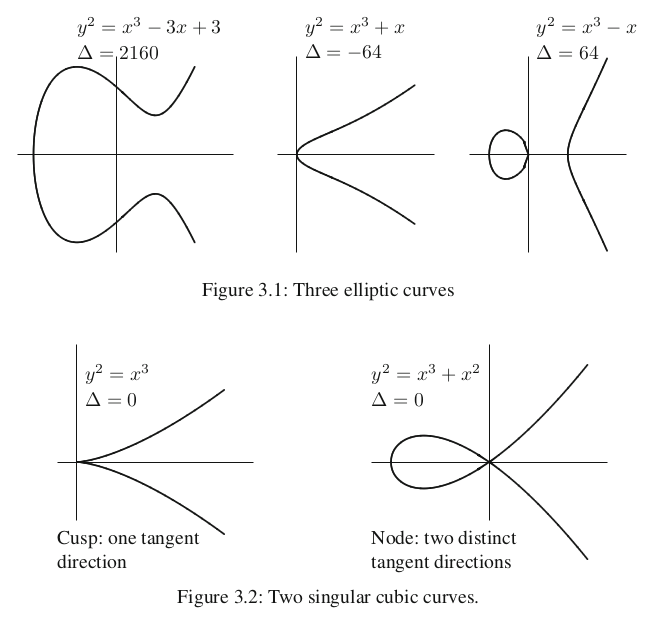
\includegraphics[width=70mm]{imagenes/curvas}
  \caption{Ejemplos de curvas elípticas ($\Delta = -16(4A^3 + 27B^2)$)}
\end{figure}
\end{frame}

\begin{frame}\frametitle{Ejemplos de curvas elípticas}
  Consideraremos las curvas elípticas sobre grupos finitos, pero ayuda
visualizarlas sobre $\mathbb{R}$ para entender las operaciones de
grupo sobre ellas. Mostramos un ejemplo de curva elíptica sobre
$\mathbb{R}$ y sobre un grupo finito.
\begin{figure}[H]
  \centering
  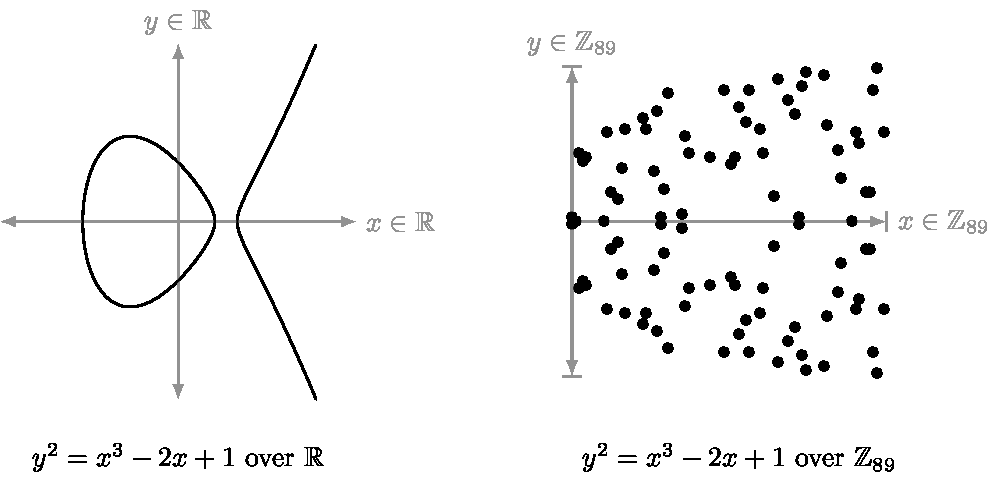
\includegraphics[width=70mm]{imagenes/curvas_Fp}
\caption{Curva elíptica sobre $\mathbb{R}$ y sobre $\mathbb{Z}_{89}$}
\end{figure}
\end{frame}

\section{Operaciones en el grupo de la curva}

\begin{frame}\frametitle{Estructura de grupo de la curva $E$}
\begin{figure}[H]
  \centering
  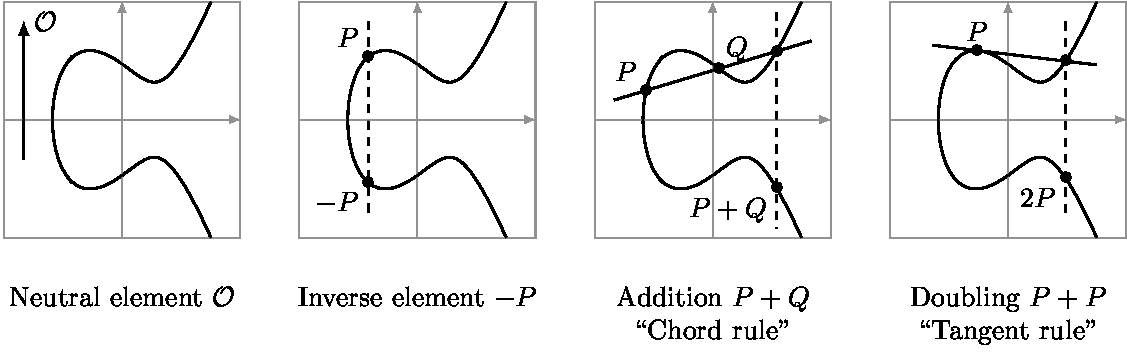
\includegraphics[width=112mm]{imagenes/operaciones}
\end{figure}

Definimos también $O+O=O$.
\end{frame}

\begin{frame}\frametitle{Estructura de grupo de la curva $E$}
\begin{figure}[H]
  \centering
  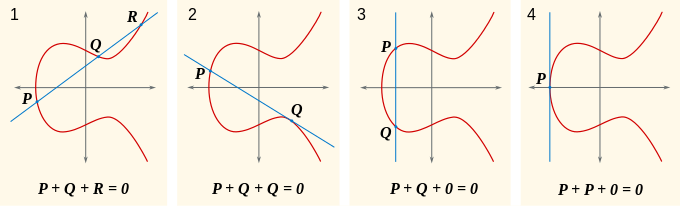
\includegraphics[width=112mm]{imagenes/suma}
\end{figure}

\begin{figure}[H]
  \centering
  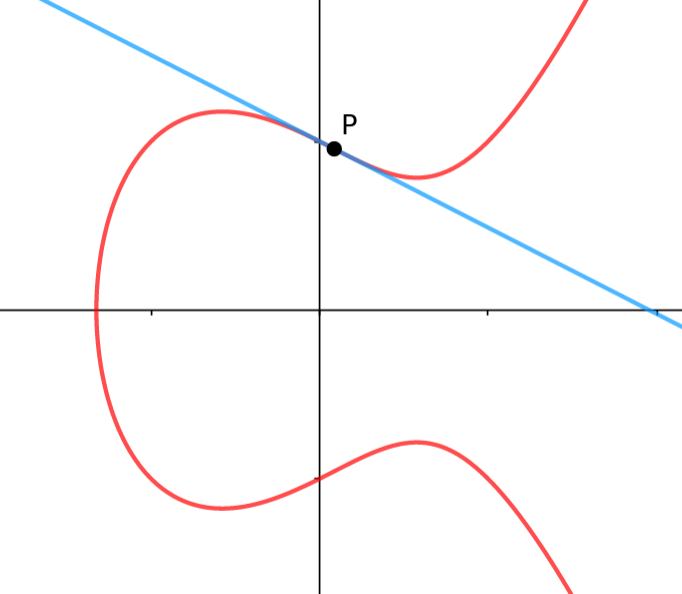
\includegraphics[width=30mm]{imagenes/suma3P}
  \caption{$P+P+P=O$}
\end{figure}
\end{frame}

\begin{frame}\frametitle{Producto por escalares}
A partir de la suma de puntos definimos el producto de un punto $P$
por un escalar $n$ como:

$$nP = \underbrace{P + P + \ldots + P}_{{n}}$$

Esta operación puede calcularse con eficiencia $O(\log n)$ escribiendo
$n$ en base $2$ y realizando duplicaciones sucesivas.
\end{frame}

\begin{frame}\frametitle{Encontrar subgrupo cíclico $<G>\subset E(\mathbb{F}_p)$}
\begin{enumerate}
\item Calculamos el número de puntos de la curva elíptica, $N =
\#E(\mathbb{F}_p)$. Esto se puede lograr mediante el
\href{https://en.wikipedia.org/wiki/Schoof\%27s_algorithm}{\color{cyan}{algoritmo de
Schoof}}.
\item Elegimos el factor primo mayor de $N$, al que llamaremos $n$.
\item Tomamos $h = N/n$. Para que una curva sea segura, el cofactor ha
de ser pequeño.
\item Escogemos un punto cualquiera de la curva $P\in E(\mathbb{F}_p)$
y sea $G=hP$.
\item Si $G$ es el punto en el infinito, cogemos otro punto $P$. De
esta manera, el orden de $G$ es $n$.
\end{enumerate}

\vfill

Podemos utilizar una curva de la \href{https://safecurves.cr.yp.to/}{\color{cyan}{lista de curvas seguras}} ya conocidas con cofactor pequeño.

\end{frame}

\section{Problema del logaritmo discreto}

\begin{frame}\frametitle{Problema del logaritmo discreto}
Sea $<G>$ un subgrupo aditivo de $E(K)$, \textbf{el problema del logaritmo
discreto} para curvas elípticas es el problema de encontrar $k$ de
manera que $kG=P$, para un punto dado $P \in <G>$.

\vspace{5mm}

La seguridad de las curvas elípticas en criptografía, descansa en la
dificultad de resolver este problema.
\end{frame}

\section{Cifrado y firma con curvas elípticas}

\begin{frame}\frametitle{Parámetros compartidos}

  Alice y Bob intercambian los siguientes parámetros por un canal potencialmente inseguro:
  
  \begin{itemize}
  \item Una curva $E(\mathbb{F}_p)$ segura.
  \item $G$ un punto de la curva de orden primo.
  \item Ambos deben conocer el valor $n$ que es el orden del grupo $<G>\subset
    E(\mathbb{F}_p)$.
  \end{itemize}
\end{frame}

\begin{frame}\frametitle{Claves pública y privada}
  Las claves son:

  \begin{itemize}
  \item Clave privada: Un entero $d_X \in [1, n-1]$ elegido de manera aleatoria.
  \item Clave pública: $Q_X=d_XG$.
  \end{itemize}

Con $X = A$ para las clavas de Alice y $X = B$ para las de Bob.

\vspace{5mm}

El cálculo de $Q_X$ se puede realizar en tiempo $O(\log d_X)$.
\end{frame}

\subsection{Algoritmo de firma digital en curvas elípticas (ECDSA)}

\begin{frame}\frametitle{Algoritmo de firma digital en curvas elípticas (ECDSA)}
  Para firmar un mensaje, Alice sigue los siguientes pasos:

\begin{enumerate}
\item Calcula $e=HASH(m)$.
\item Si definimos $L_n$ como el número de bits de $n$, toma $z$ los $L_n$ bits menos
significativos de $e$.
\item Elige de manera aleatoria un entero secreto $k \in [1,n-1]$.
\item Calcula el punto de la curva $(x_1, y_1)=kG$.
\item Toma $r = x_1 \text{ mod }n$. En el caso de que $r$ sea 0,
vuelve al paso 3.
\item Calcula $s=k^{-1}(z+rd_A) \text{ mod }n$. Si $s$ es 0, vuelve al paso 3.
\end{enumerate}

La firma es el par $(r,s)$.
\end{frame}

\begin{frame}\frametitle{Verificación de la firma}

  Para verificar que el emisor es Alice, Bob seguirá los pasos siguentes:
  \begin{enumerate}
\item Comprueba que $Q_A \neq O$.
\item Se debe cumplir que $nQ_A=O$
\end{enumerate}

Si las comprobaciones anteriores son satisfactorias, Bob deberá
entonces proceder de la siguiente manera:

\begin{enumerate}
\item Comprueba que $r,s\in[1, n-1]$, en otro caso, la firma es
inválida.
\item Calcula  $e$ usando la misma función de hashing que uso Alice.
\item Toma de nuevo $z$ los $L_n$ bits menos significativos de $e$.
\item Obtiene $u_1 = zs^{-1} \text{ mod } n$ y $u_2 = rs^{-1} \text{
mod } n$.
\item Calcula el punto $C = (x_1,y_1)=u_1G+u_2Q_A$. Si $(x_1,
y_1)=O$ entonces la firma no es válida.
\end{enumerate}
Finalmente la firma será válida si $r = x_1 \text{ mod }n$. En caso contrario, no lo será.
\end{frame}

\begin{frame}\frametitle{Comprobación de los pasos de Bob}
Veremos por qué con $C=u_1G+u_2Q_A$ obtenemos el resultado que queremos. Para ello notamos en primer lugar que $Q_A=d_AG$ por lo que
$$C=u_1G+u_2d_AG$$
Ahora usamos la propiedad asociativa:
$$C = (u_1+u_2d_A)G$$
desarrollamos las expresiones de $u_1$ y $u_2$
$$C = (zs^{-1}+rd_As^{-1})G$$
y aplicamos la propiedad asociativa de nuevo con lo que
$$C = (z+rd_A)s^{-1}G$$
Sustituimos $s$ por su expresión tal y como se calculó en el
algoritmo:
$$C = (z+rd_A)(z+rd_A)^{-1}(k^{-1})^{-1}G$$
con lo que obtenemos $C = kG$
\end{frame}

\begin{frame}\frametitle{Problema}
\end{frame}

\begin{frame}\frametitle{}
\end{frame}

\begin{frame}[fragile]\frametitle{Simulación}
  \begin{lstlisting}
    Recuerda poner fragile en el cógigo
  \end{lstlisting}
\end{frame}

\end{document}